\documentclass[handout]{beamer}
% \documentclass{beamer}

%%
%%
%%
% From http://tex.stackexchange.com/questions/2072/beamer-navigation-circles-without-subsections
% Solution #2 or 3:
% \usepackage{etoolbox}
% \makeatletter
% % replace the subsection number test with a test that always returns true
% \patchcmd{\slideentry}{\ifnum#2>0}{\ifnum2>0}{}{\@error{unable to patch}}%
% \makeatother
% Solution #1:
\usepackage{remreset}% tiny package containing just the \@removefromreset command
\makeatletter
\@removefromreset{subsection}{section}
\makeatother
\setcounter{subsection}{1}


\usepackage{etex}
\usepackage{pgf}
\usepackage{tikz}
\usepackage{url}
\usepackage{amsmath}
\usepackage{color}
% \definecolor{red}{rgb}{1,0,0}
\usepackage{ulem}
% \usepackage{booktabs}
\usepackage{colortbl,booktabs}
\renewcommand*{\thefootnote}{\fnsymbol{footnote}}
\usepackage{fancybox}
\usepackage[framemethod=TikZ]{mdframed}
\mdfdefinestyle{FactStyle}{%
  outerlinewidth=0.5,
  roundcorner=1pt,
  leftmargin=1cm,
  linecolor=blue,
  outerlinecolor=blue!70!black,
  backgroundcolor=yellow!40
}
\usepackage{cancel}

  \newcommand\Warning{%
    \makebox[2.4em][c]{%
      \makebox[0pt][c]{\raisebox{.2em}{\Large!}}%
      \makebox[0pt][c]{\color{red}\Huge$\bigtriangleup$}}}%

\usepackage{stackengine}
\usepackage{scalerel}
\usepackage{xcolor}
  \newcommand\dangersign[1][2ex]{%
    \renewcommand\stacktype{L}%
    \scaleto{\stackon[1.3pt]{\color{red}$\triangle$}{\tiny !}}{#1}%
  }



\usepackage{dcolumn}
\newcolumntype{d}[1]{D{.}{.}{#1}}

% From
% http://tex.stackexchange.com/questions/109900/how-can-i-box-multiple-aligned-equations
\usepackage{empheq}
\usepackage{tcolorbox}  \newtcbox{\othermathbox}[1][]{%
  nobeforeafter, tcbox raise base, 
  colback=black!10, colframe=red!30, 
  left=1em, top=0.5em, right=1em, bottom=0.5em}

\newcommand\blue{\color{blue}}
\newcommand\red{\color{red}}
\newcommand\green{\color{green!75!black}}
\newcommand\purple{\color{purple}}
\newcommand\bluegreen{\color{blue!75!green}}
\newcommand\orange{\color{orange}}
\newcommand\redgreen{\color{red!50!green}}
\newcommand\grey{\color{black}}
\newcommand\gap{\vspace{.1in}}
\newcommand\nb{${\red\bullet}\ $}
\newcommand\halfgap{\vspace{.05in}}
\newcommand\divideline{\line(1,0){352}}
\usepackage{marvosym} % for \Smiley

\newcommand{\bluealert}[1]{{\blue\textbf{#1}}}

% \usepackage{beamerthemesplit} %Key package for beamer
\usetheme{Singapore}
% \usetheme{Szeged}
% \usetheme{Garfield}
% \usetheme{CambridgeUS}
% \usenavigationsymbolstemplate{} %Gets rid of slide navigation symbols


\setbeamercolor{separation line}{use=structure,bg=structure.fg!50!bg}
% \begin{beamercolorbox}[colsep=0.5pt]
%   {upper separation line foot}
% \end{beamercolorbox}



\makeatletter
\setbeamertemplate{footline}
{
  \leavevmode%
  \hbox{%
% \begin{beamercolorbox}[colsep=0.5pt]
%   {upper separation line foot}
% \end{beamercolorbox}


  \begin{beamercolorbox}[wd=.5\paperwidth,ht=2.25ex,dp=2ex,colsep=0.5pt]%
    {upper separation line foot}
    \usebeamerfont{author in head/foot}%
    \hspace*{2ex}\insertshortdate:\ \insertshorttitle
  \end{beamercolorbox}%
  \begin{beamercolorbox}[wd=.5\paperwidth,ht=2.25ex,dp=2ex,right]{title in head/foot}%
    \usebeamerfont{title in head/foot}
    {\insertshortauthor}\hspace*{2ex}
  \end{beamercolorbox}}%
  % \begin{beamercolorbox}[wd=.333333\paperwidth,ht=2.25ex,dp=2ex,right]{date in head/foot}%
  %   \usebeamerfont{date in head/foot}\insertshortdate{}\hspace*{2em}
  %   \insertframenumber{} / \inserttotalframenumber\hspace*{2ex} 
  % \end{beamercolorbox}%
  \vskip0pt%
}
\makeatother

\usetikzlibrary{decorations.markings}
\usetikzlibrary{arrows}


\title{Final Exam Review}
\author{Peter Garfield, UCSB Mathematics}
\date{March 15, 2017}
%\institute{}


\useinnertheme{default}

\usefonttheme{serif}
% \usecolortheme{rose}
% \usecolortheme{whale}
% \usecolortheme{orchid}
\usecolortheme{crane}
% \usecolortheme{dolphin}


%TEMPLATE
\setbeamertemplate{navigation symbols}{}

\setbeamertemplate{note page}[compress]

\setbeamertemplate{frametitle}{
  \vspace{0.5em}
  % \begin{centering}
  {\huge\blue\textbf{\textmd{\insertframetitle}}}
  \par
  % \end{centering}
}

% From http://tex.stackexchange.com/questions/7032/good-way-to-make-textcircled-numbers:
\newcommand*\circled[1]{\tikz[baseline=(char.base)]{\node[shape=circle,draw,fill=orange,inner sep=1pt] (char) {#1};}} 
% \renewcommand{\labelenumi}{\circled{\textbf{\arabic{enumi}}}}

\let\olddescription\description
\let\oldenddescription\enddescription
\usepackage{enumitem}
\let\description\olddescription
\let\enddescription\oldenddescription

% \usepackage[loadonly]{enumitem}
\setlist[enumerate,1]{label=\colorbox{orange}{\arabic*.},font=\bfseries}
%\setlist[enumerate,2]{label=\colorbox{blue!25}{(\alph*)},font=\bfseries}
% \setlist[enumerate,1]{label=\arabic*.,font=\bfseries}
\setlist[itemize,1]{label=\red$\bullet$}
\setlist[itemize,2]{label=\blue$\bullet$}

\newcommand\answer[1]{\fbox{#1}}
% \renewcommand\answer[1]{}

\newcommand{\antilog}{\operatorname{antilog}}







\title{}
\title{All About Lines}
\date{April 14, 2017}


\begin{document}
\small

\section*{Administration}

\frame{
  \frametitle{Office Hours!}
  % \ \vspace*{0.25in}

  {\Large{}Instructor:}\\
  \ \hspace*{0.2in} Trevor Klar, \url{trevorklar@math.ucsb.edu}\\[0.25em]

  {\Large{}Office Hours:}\\
  \ \hspace*{0.2in} Mondays 2--3\textsc{pm}\\
  \ \hspace*{0.2in} Tuesdays 10:30--11:30\textsc{am}\\
  \ \hspace*{0.2in} Thursdays 1--2\textsc{pm}\\
  \ \hspace*{0.2in} or by appointment \\[0.25em]

  {\Large{}Office:}\\
  \ \hspace*{0.2in} South Hall 6431X (Grad Tower, 6th floor, blue side, first door on the right)\\[0.5em]

  \copyright\ 2017\ Daryl Cooper, Trevor Klar

  % \vspace*{2in}
}

\frame{
  \frametitle{Exam 1: Wednesday in class}

  {\Large\color{blue}Bring:}
  \begin{itemize}
  \item A blue book
  \item A $3"\times5"$ card (both sides!) with your notes.
  \item A pen / pencil
  \item An ID
  \end{itemize}
  \bigskip

  {\Large\color{red}Don't bring:}
  \begin{itemize}
  \item A calculator
  \end{itemize}
  \bigskip

  {\Large\color{orange}Please Be Early!}
  \smallskip

  See Gauchospace and textbook for sample exams.


}

\section*{Lines}


\frame{
  \frametitle{Straight Lines (\S 6.1)}

  \alert{The Slope Intercept Form}\ 

  The \textbf{slope intercept}\ equation of a straight line is \ \fbox{$y = {\color{blue}m}x + {\color{red}b}$}\,.

  \begin{center}
    \begin{tikzpicture}[x=8mm,y=6mm,>=latex]
      \draw[thin,black,->] (-3,0) -- (7,0) node[below] {$x$};
      \draw[thin,black,->] (0,-0.5) -- (0,5) node[left] {$y$};
      % y=-2+(3/4)*(x+2) or y=3/4 x - 1/2 = (3x-2)/4
      % m=5/10 = 1/2, so y=4+(1/2)*(x-6) or y=x/2+1:
      \draw[thick,black] (-3,-0.5) -- (7,4.5) node[right] {$y=mx+b$};
      \filldraw[red] (0,1) circle (1.5pt) node[red,left,yshift=1.5mm] {$b$};
    \end{tikzpicture}
  \end{center}
  \vspace*{-1.5em}

  \begin{align*}
    {\color{blue}m} & = \text{the \textbf{slope}.  CRUCIAL for calculus.} \\
    {\color{red}b}  & =\, \text{where the line crosses\ the $y$-axis (the ``$y$-intercept'').}
  \end{align*}
  \pause  
  WHY? Because when you plug in $x=0$, you get $y={\color{red}b}$.

}

\frame{
  \frametitle{Example}

  \begin{enumerate}
  \item Find the equation of the line \fbox{$y={\blue m}x+{\red b}$}
    through the points $(1,3)$ and $(7,5)$.  
    \bigskip

    Plan: Find $m$, then find $b$.
    \bigskip
    \pause

    \begin{enumerate}
    \item  What is $m$?
      \begin{center}
        A$=1$
        \quad 
        B$=3$
        \quad 
        C$=5$
        \quad 
        D$=1/3$
        \quad 
        E$=2$
        \quad
        \pause
        \fbox{D}
      \end{center}
      \bigskip
      \pause

      So $\displaystyle{}y=\frac{1}{3}x + b$.  What is $b$?  Plug in
      either point!
      \bigskip
      
      \item What do you get for ${\red b}$?
        \begin{center}
          A$=1/3$
          \quad 
          B$= 4/3$
          \quad 
          C$= 7/3$
          \quad 
          D$= 8/3$
          \quad
          E$= 10/3$ 
          \pause
          \quad
          \fbox{D}
        \end{center}

        \halfgap

        \item Can we check?
    \end{enumerate}
  \end{enumerate}
    
}

\frame{
  \frametitle{You Try It}

  \begin{enumerate}
    \setcounter{enumi}{1}
  \item A line has slope $1/2$ and goes through the point $(2,5).$
    What is the $y$-coordinate of the point on this line where $x=6$?
    \bigskip
    \begin{center}
      A$=3$
      \qquad 
      B$=4$
      \qquad 
      C$=5$
      \qquad 
      D$=6$
      \qquad 
      E$=7$ 
      \quad
      \uncover<3->{\fbox{E}}
    \end{center}
    \pause
    \bigskip

    \uncover<2->{%
      \alert{Plan:}\ 
      \parbox[t]{2in}{%
        1.\ Find equation of the line. \\
        2.\ Plug in $x=6$ to find $y$.
      }
    }
  \end{enumerate}
  \vspace*{1in}
  \ 
}

\frame{
  \frametitle{Another Equation of a Line}

  \alert{The Point-Slope Form}\ 

  The \textbf{point slope}\ equation of a straight line is \ \fbox{$y = {\color{red}y_0}+{\color{blue}m}(x - {\color{red}x_0})$}\,.

  \begin{center}
    \begin{tikzpicture}[x=8mm,y=6mm,>=latex]
      \draw[thin,black,->] (-3,0) -- (7,0) node[below] {$x$};
      \draw[thin,black,->] (0,-0.5) -- (0,5) node[left] {$y$};
      % y=-2+(3/4)*(x+2) or y=3/4 x - 1/2 = (3x-2)/4
      % m=5/10 = 1/2, so y=4+(1/2)*(x-6) or y=x/2+1:
      \draw[thick,black] (-3,-0.5) -- (7,4.5);% node[right] {$y=mx+b$};
      \filldraw[red] (2,2) circle (1.5pt) node[red,above,xshift=-2.5mm] {\small$(x_0,y_0)$};
      \draw[red,thin,dotted] (2,2) -- (2,0) node[below] {$x_0$};
      \draw[red,thin,dotted] (2,2) -- (0,2) node[left] {$y_0$};
    \end{tikzpicture}
  \end{center}
  \vspace*{-1.5em}

  \begin{align*}
    {\color{blue}m} & = \text{the \textbf{slope}.  Still CRUCIAL for calculus.} \\
    {\color{red}(x_0,y_0)}  & =\, \text{any point on the line.}
  \end{align*}

}

\frame{
  \frametitle{Why Does This Work?}

  \begin{center}
    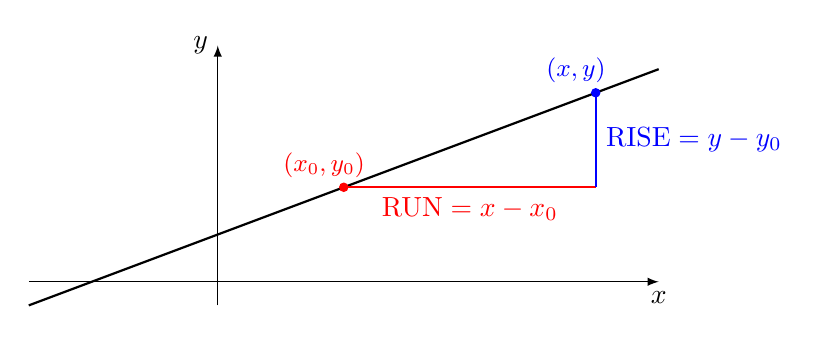
\begin{tikzpicture}[x=8mm,y=6mm,>=latex]
      \draw[thin,black,->] (-3,0) -- (7,0) node[below] {$x$};
      \draw[thin,black,->] (0,-0.5) -- (0,5) node[left] {$y$};
      % y=-2+(3/4)*(x+2) or y=3/4 x - 1/2 = (3x-2)/4
      % m=5/10 = 1/2, so y=4+(1/2)*(x-6) or y=x/2+1:
      \draw[thick,black] (-3,-0.5) -- (7,4.5);
      \filldraw[red] (2,2) circle (1.5pt) node[red,above,xshift=-2.5mm] {\small$(x_0,y_0)$};
      \uncover<2->{%
        \filldraw[blue] (6,4) circle (1.5pt) node[above,xshift=-2.5mm] {\small$(x,y)$};
        \draw[thick,red] (2,2) -- (6,2) node[midway,below]{$\text{RUN}=x-x_0$};
        \draw[thick,blue] (6,2) -- (6,4) node[midway,right]{$\text{RISE}=y-y_0$};
      }
      % \draw[red,thin,dotted] (2,2) -- (2,0) node[below] {$x_0$};
      % \draw[red,thin,dotted] (2,2) -- (0,2) node[left] {$y_0$};
    \end{tikzpicture}
  \end{center}
  \vspace*{-1.5em}

  \begin{align*}
    \text{$(x,y)$ lies on the line}
    & \ \text{exactly when} 
    && \uncover<3->{\frac{y-y_0}{x-x_0} = m} \\
    &&& \uncover<4->{y-y_0 = m(x-x_0)} \\
    &&& \uncover<5->{y=y_0 + m(x-x_0)}
  \end{align*}

}

\frame{
  \frametitle{Examples}

  \begin{enumerate}
    \setcounter{enumi}{2}
  \item Find the equations of these lines (whose slopes we've already
    found):
  \end{enumerate}

  \begin{center}
    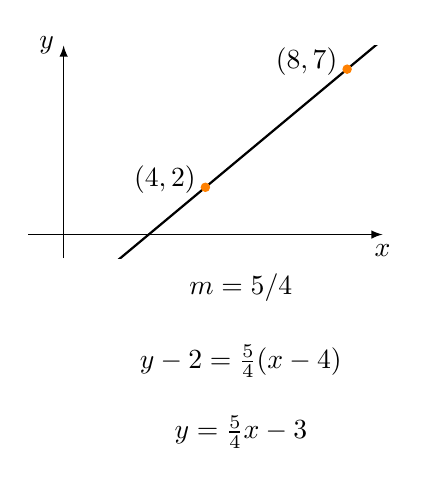
\begin{tikzpicture}[x=4.5mm,y=3mm,>=latex]
      \draw[thin,black,->] (-1,0) -- (9,0) node[below] {$x$};
      \draw[thin,black,->] (0,-1) -- (0,8) node[left] {$y$};
      \begin{scope}
        \clip (-1,-1) rectangle (9,8);
        % line thru (4,2) and (8,7):
        \draw[thick,black] plot[domain=-1:9] (\x,{2+5*(\x-4)/4});
      \end{scope}
      \filldraw[orange] (4,2) circle (1.5pt) node[black,left,yshift=1mm] {$(4,2)$};
      \filldraw[orange] (8,7) circle (1.5pt) node[black,left,yshift=1mm] {$(8,7)$};
      \node[below] at (5,-1.25) {$m=5/4$};
      \uncover<2->{%
        \node[below] at (5,-4.25) {$y-2=\frac{5}{4}(x-4)$};
      }
      \uncover<3->{%
        \node[below] at (5,-7.25) {$y=\frac{5}{4}x-3$};
      }
    \end{tikzpicture}
    \hspace*{6mm}
    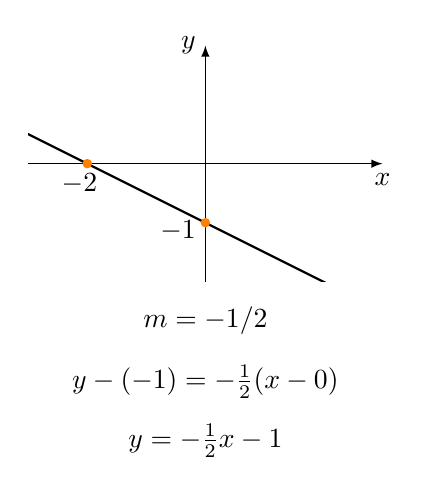
\begin{tikzpicture}[x=7.5mm,y=7.5mm,>=latex]
      \draw[thin,black,->] (-3,0) -- (3,0) node[below] {$x$};
      \draw[thin,black,->] (0,-2) -- (0,2) node[left] {$y$};
      \begin{scope}
        \clip (-3,-2) rectangle (3,2);
        % line thru (-2,0) and (0,-1):
        \draw[thick,black] plot[domain=-4:6] (\x,{-1*\x/2-1});
      \end{scope}
      \filldraw[orange] (-2,0) circle (1.5pt) node[black,below,xshift=-1mm] {$-2$};
      \filldraw[orange] (0,-1) circle (1.5pt) node[black,left,yshift=-1mm] {$-1$};
      \node[below] at (0,-2.25) {$m=-1/2$};
      \uncover<4->{%
        \node[below] at (0,-3.25) {$y-(-1)=-\frac{1}{2}(x-0)$};
      }
      \uncover<5->{%
        \node[below] at (0,-4.25) {$y=-\frac{1}{2}x-1$};
      }
    \end{tikzpicture}
  \end{center}


}


\frame{
  \frametitle{And\ldots?}

  Yes, but what's this got to do with calculus?\\ \pause
  {\red Derivatives} are about \textbf{\color{blue}rate of change}
  and that is what {\blue\textbf{slope}}\ is!\\ \pause
  \gap

  \alert{Example:}\ This graph shows the temperature in an oven as it heats up:
  \begin{center}
    % \includegraphics[scale=0.7]{lines7small} 
    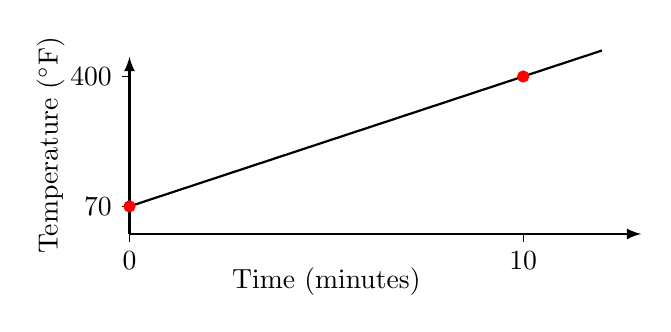
\begin{tikzpicture}[x=5mm,y=0.05mm,>=latex]
      \draw[thick,black,->] (0,0) -- (13,0);
      \draw[thick,black,->] (0,0) -- (0,450);
      \node at (5,-120) {Time (minutes)};
      \node[rotate=90] at (-2,225) {Temperature (${}^{\circ}\text{F}$)};
      \foreach \x in {0,10} 
      {
        \draw[thin,black] (\x,0) -- (\x,-1mm) node[below] {$\x$};
      }
      \foreach \y in {70,400} 
      {
        \draw[thin,black] (0,\y) -- (-1mm,\y) node[left] {$\y$};
      }
      \draw[thick,black] (0,70) -- (12,{70+33*12});
      \filldraw[red] (0,70) circle (2pt);
      \filldraw[red] (10,400) circle (2pt);
    \end{tikzpicture}
  \end{center}
  \vspace*{-0.1in}
  \pause

  \begin{enumerate}
    \setcounter{enumi}{3}
  \item  How quickly (in {\red ${}^{\circ}\text{F}/\text{min}$})\ is
    the oven heating up? 
    \begin{center}
      A$=70$
      \quad 
      B$=10$
      \quad 
      C$=40$
      \quad 
      D$=33$
      \quad 
      E$=$Other
      \qquad\pause\fbox{D}
    \end{center}
  \end{enumerate}
  \bigskip
  \pause

  Moral:  \vspace*{-0.35in}

  \begin{empheq}[box=\othermathbox]{equation*}
    \text{{\color{red}Rate of increase}}
    = 
    \text{{\color{blue}\textbf{slope}}}
  \end{empheq}
 
} 


\frame{
  \frametitle{One More Example}

  \begin{enumerate}
    \setcounter{enumi}{4}
  \item Where does the line $y=1+x$ cross the line $y=3-x$?\\
    Find both the $x$ and $y$ coordinates of the crossing point.\\
  \end{enumerate}
  \bigskip
  \pause
  
  Plan:
  \begin{enumerate}
  \item[1.]  \alert{Draw a picture!}\ showing two straight lines crossing.
  \item[2.] Solve the {\red two simultaneous equations}
  \item[3.] {\green THINK} why this gives the answer!
  \end{enumerate}
  % \vspace*{2in}
  \pause

  \begin{center}
    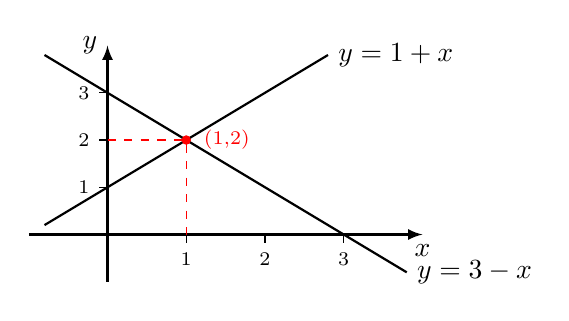
\begin{tikzpicture}[x=10mm,y=6mm,>=latex]
      \draw[thick,black,->] (-1,0) -- (4,0) node[below] {$x$};
      \draw[thick,black,->] (0,-1) -- (0,4) node[left] {$y$};
      \foreach \k in {1,2,3}
      {
        \draw[thin,black] (\k,0) -- (\k,-3pt) node[below] {$\scriptstyle\k$};
        \draw[thin,black] (0,\k) -- (-3pt,\k) node[left] {$\scriptstyle\k$};
      }
      % y=1+x:
      \draw[thick,black] (-0.8,0.2) -- (2.8,3.8) node[right] {$y=1+x$};
      % y=3-x:
      \draw[thick,black] (-0.8,3.8) -- (3.8,-0.8) node[right] {$y=3-x$};
      \draw[thin,red,dashed] (0,2) -- (1,2) -- (1,0);
      \filldraw[red] (1,2) circle (1.5pt) node[right,xshift=1mm] {$\scriptstyle(1,2)$};
    \end{tikzpicture}
  \end{center}
}

\section*{Applications}

\frame{
  \frametitle{Linear Interpolation}%\ (predicting the past)}
  % {\purple Section (6.3) Linear Interpolation} (predicting the past)

  \begin{enumerate}
    \setcounter{enumi}{5}
  \item In 2000, a population was $1000$.  In 2010, it was $1100$.
    What would you \alert{\emph{guess}}\ the population was in 2005?
    \begin{center}
      A$=1005$
      \quad 
      B$ = 1020$
      \quad 
      C$ = 1050$
      \quad
      D$ = 2050$
      \quad 
      E$ =2010$ 
      \quad
      \pause
      \fbox{C}    
    \end{center}
  \end{enumerate}

  \begin{center}
    % \includegraphics[scale=0.7]{pop2a.pdf}
    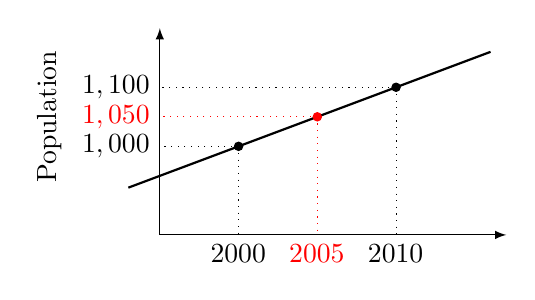
\begin{tikzpicture}[x=2.0mm,y=0.075mm,>=latex]
      \draw[thin,black,->] (1995,850) -- (2017,850);
      \draw[thin,black,->] (1995,850) -- (1995,1200);
      \draw[thick,black] plot[domain=1993:2016] (\x,{1000+10*(\x-2000)});
      \draw[thin,black,dotted] (2000,1000) -- (1995,1000) node[left] {$1,000$};
      \draw[thin,black,dotted] (2010,1100) -- (1995,1100) node[left] {$1,100$};
      \draw[thin,black,dotted] (2000,1000) -- (2000,850) node[below] {2000};
      \draw[thin,black,dotted] (2010,1100) -- (2010,850) node[below] {2010};
      \filldraw[black] (2000,1000) circle (1.5pt);
      \filldraw[black] (2010,1100) circle (1.5pt);
      \node[rotate=90] at (1988,1050) {Population};
      \uncover<4->{%
        \draw[thin,red,dotted] (2005,1050) -- (1995,1050) node[left] {$1,050$};
        \draw[thin,red,dotted] (2005,1050) -- (2005,850) node[below] {2005};
        \filldraw[red] (2005,1050) circle (1.5pt);
      }
    \end{tikzpicture}
  \end{center}
  
  This is a \alert{\emph{guess}}\ \pause{}based on the assumption that
  population grows at a \alert{\emph{constant rate}}.
  \pause

  ``\alert{Constant rate}''\ means that the graph of population is a \emph{straight line}.


}

\frame{
  \frametitle{Linear Extrapolation}%\ (predicting the future)}
  % {\color{blue}Section (6.3) Linear Extrapolation} (predicting the future)

  \begin{enumerate}
    \setcounter{enumi}{6}
  \item In 2000, a population was $1000$.  In 2010, it was $1100$.
    What would you \alert{\emph{guess}}\ the population will be in
    2020?

    \begin{center}
      A$=1150$
      \quad 
      B$ = 1200$
      \quad 
      C$ = 1250$
      \quad
      D$ = 2020$
      \quad 
      E$ = $Other 
      \quad
      \pause
      \fbox{B}    
    \end{center}
  \end{enumerate}

  \begin{center}
    % \includegraphics[scale=0.7]{pop2a.pdf}
    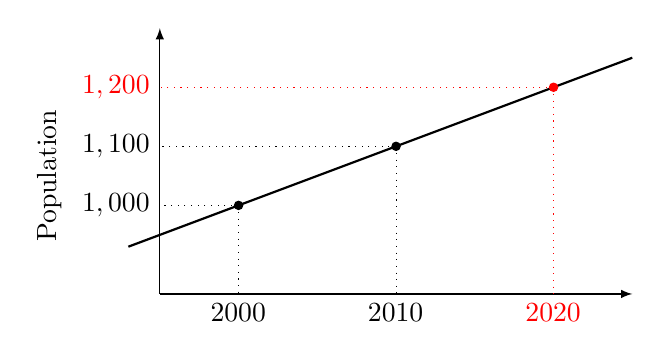
\begin{tikzpicture}[x=2.0mm,y=0.075mm,>=latex]
      \draw[thin,black,->] (1995,850) -- (2025,850);
      \draw[thin,black,->] (1995,850) -- (1995,1300);
      \draw[thick,black] plot[domain=1993:2025] (\x,{1000+10*(\x-2000)});
      \draw[thin,black,dotted] (2000,1000) -- (1995,1000) node[left] {$1,000$};
      \draw[thin,black,dotted] (2010,1100) -- (1995,1100) node[left] {$1,100$};
      \draw[thin,black,dotted] (2000,1000) -- (2000,850) node[below] {2000};
      \draw[thin,black,dotted] (2010,1100) -- (2010,850) node[below] {2010};
      \filldraw[black] (2000,1000) circle (1.5pt);
      \filldraw[black] (2010,1100) circle (1.5pt);
      \node[rotate=90] at (1988,1050) {Population};
      \uncover<4->{%
        \draw[thin,red,dotted] (2020,1200) -- (1995,1200) node[left] {$1,200$};
        \draw[thin,red,dotted] (2020,1200) -- (2020,850) node[below] {2020};
        \filldraw[red] (2020,1200) circle (1.5pt);
      }
    \end{tikzpicture}
  \end{center}
  
  Again: a \alert{\emph{guess}}\ \pause{}based on the assumption that
  population grows at a \alert{\emph{constant rate}}.


}


\frame{
  \frametitle{A Problem}
  
  You can't tell someone you just ``\alert{guessed}''\ the answer or
  just ``\alert{drew a straight line}''.  You need to make it
  \emph{sound}\ more ``\alert{scientific}'' so give it a complicated
  sounding name to impress people.  
  \pause 
  \gap

  {\blue Linear Interpolation} and {\blue Linear Extrapolation}. 
  \halfgap

  {\blue Linear} means straight line\\
  {\blue inter} means {\blue between} like {\blue inter}city\\
  {\blue extra} means {\blue beyond} like  {\blue extra}ordinary\\
  % {\blue -polation} to do with numbers
  \gap

  % {\blue interpolate }\quad
  % from Latin {\blue interpolare} ``alter, freshen up, {\red falsify}''
  % \pause
  % \gap 

  The {\red idea} is to {\blue assume} the population (or whetever)
  {\blue grows at a constant rate}.\\ 
  Then use this to predict. \pause
  \gap

  {\blue Method:}\\
  {\blue (1)}\ Use given data to draw a straight line and find equation $y=mx+b$\\
  {\blue (2)}\ Use the equation to make predictions.

}

\frame{ 
  \frametitle{Wiktionary: interpolo (Latin)}

  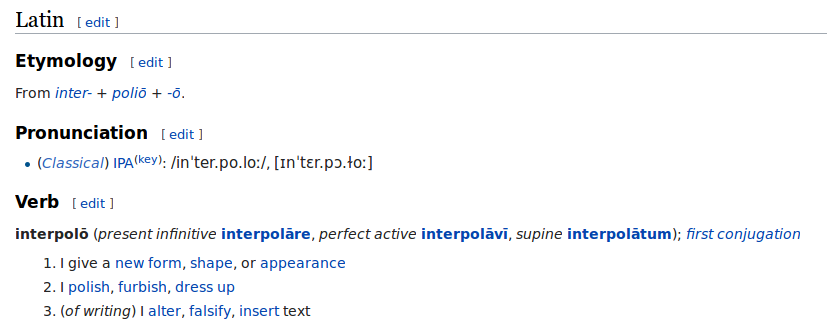
\includegraphics[width=\textwidth]{wiktionary-interpolo}
}


\frame{
  \frametitle{Linear Extrapolation}%\ (predicting the future)}
  % {\color{blue}Section (6.3) Linear Extrapolation} (predicting the future)

  \begin{enumerate}
    \setcounter{enumi}{7}
  \item In 2000, a population was $1000$.  In 2010, it
    was $1100$.  Let
    \begin{align*}
      x & =\text{number of years after 2000 (Ex: $x=3$ is the year 2003)}\\
      y & =\text{population in the year $x$}
    \end{align*}
    Find the equation of a line $y=mx+b$:
  \end{enumerate}
  \begin{center}
      A:\ $2000+1000x$
      \ \ 
      B:\ $1000+2000x$
      \ \ 
      C:\ $1000+100x$
      \ \ 
      D:\ $1000+10x$
  \end{center}
  \only<2>{\alert{Answer:}\ \answer{D}}
  \vspace*{-0.1in}

  \uncover<3->{%
    \begin{center}
      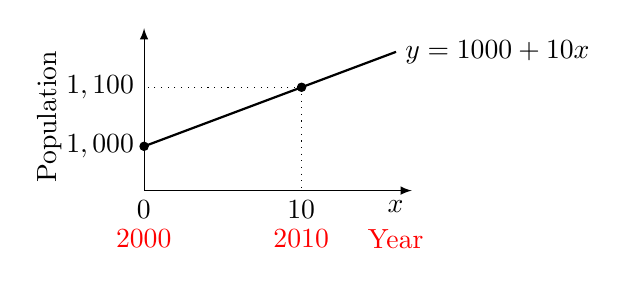
\begin{tikzpicture}[x=2.0mm,y=0.075mm,>=latex]
        \draw[thin,black,->] (2000,925) -- (2017,925);
        \draw[thin,black,->] (2000,925) -- (2000,1200);
        \draw[thick,black] plot[domain=2000:2016] (\x,{1000+10*(\x-2000)});
        \node[left] at (2000,1000) {$1,000$};
        \draw[thin,black,dotted] (2010,1100) -- (2000,1100) node[left] {$1,100$};
        \node[below] at (2000,925) {$0$};
        \node[below] at (2016,925) {$x$};
        \draw[thin,black,dotted] (2010,1100) -- (2010,925) node[below] {$10$};
        \filldraw[black] (2000,1000) circle (1.5pt);
        \filldraw[black] (2010,1100) circle (1.5pt);
        \node[rotate=90] at (1994,1050) {Population};
        \uncover<4->{%
          % \draw[thin,red,dotted] (2005,1050) -- (1995,1050) node[left] {$1,050$};
          % \draw[thin,red,dotted] (2005,1050) -- (2005,925) node[below] {2005};
          % \filldraw[red] (2005,1050) circle (1.5pt);
          \node[right] at (2016,1160) {$y=1000+10x$};
          \node[red,below] at (2000,875) {2000};
          \node[red,below] at (2010,875) {2010};
          \node[red,below] at (2016,875) {Year};
        }
      \end{tikzpicture}
    \end{center}
  }
  \vspace*{-0.1in}

  \uncover<5->{%
    \begin{enumerate}
      \setcounter{enumi}{8}
    \item When will population be 1350?
    \end{enumerate}
    \begin{center}
      A$=2015$
      \quad 
      B$=2025$
      \quad 
      C$=2035$
      \quad 
      D$=3350$
      \quad 
      E$=$Other
      \quad
      \uncover<6->{\fbox{C}}
    \end{center}
  }
}


\frame{
  \frametitle{Another Example}

  \begin{enumerate}
    \setcounter{enumi}{9}
  \item The number of unemployed in LA on January 1, 2015 was
    $50,000$.  After 100 days, it was $45,000$.
  \smallskip

  \begin{enumerate}
  \item Estimate the number of unemployed $300$ days after Jan.\ 1.
  \begin{center}
    \hspace*{-0.5in}
    \mbox{
      A$= 40,000$
      \quad 
      B$= 35,000$
      \quad 
      C$= 30,000$
      \quad 
      D$= 25,000$
      \quad 
      E$= 300$
      \pause
      \quad
      \fbox{B}
    }
  \end{center}
  \bigskip
  % {\color{blue}  MAYBE.} \pause
  % \quad This is a {\purple prediction}.\pause\  You can't expect it to be very accurate!!!\\ \pause
  % {\blue "Prediction is very difficult, especially if it's about the future."}\\

  % {\red Nils Bohr}, Nobel laureate in Physics\\ \pause
  \halfgap

  \item Suppose
    \vspace*{-2em}
    \begin{align*}
      \ \qquad x & = \text{the number of days after January 1}\\
      y & = \text{number of unemployed people on day $x$.}
    \end{align*}
    Then the equation of the line used for this linear extrapolation is $y=$
    \vspace*{-1em}
    \begin{center}
      \mbox{
        A$=-100+50,000x$
        \quad 
        B$=50,000-100x$
        \quad 
        C$=45,000-100x$
      }

      \mbox{
        D$=50,000-50x$
        \quad 
        E$=45,000-50x$
        \pause
        \quad 
        \fbox{D}
      }
    \end{center}
    \halfgap

  \item How many days until unemployed reaches $30,000$?
  \begin{center}
    A$=40$
    \quad 
    B$=140$
    \quad
    C$=200$
    \quad 
    D$=300$
    \quad 
    E$=400$
    \quad
    \pause
    \fbox{E}
  \end{center}
  \end{enumerate}
\end{enumerate}

}


\frame{
  \frametitle{Proportionality}
  % \vspace{.1in}
  % {\bf \color{blue}(6.2) Proportionality}\\

  {\large\blue{}Simple Idea:}\ $y\propto x$\quad ``$y$ is proportional to $x$''
  means:
  \begin{empheq}[box=\othermathbox]{equation*}
    \text{If you double $x$, then $y$ doubles. Triple $x$ then $y$
      triples. And so on.}
  \end{empheq}

  \alert{Example:}\ \ 
  If you are paid by the hour then
  \begin{center}
    (amount you earn) $\ \propto\ $ (number of hours you work)
  \end{center}
  \halfgap

  If you work for $10$ hours, then you are paid \$$50$. 
  How much are you paid if you work for $20$ hours?
  \begin{center}
    A$ = \$20$
    \quad 
    B$ = \$50$
    \quad 
    C$ = \$200$
    \quad 
    D$ = \$100$
    \quad 
    E=Other
    \quad
    \pause{\fbox{D}}
  \end{center}
  % You work twice as many hours ($20 = 2\times 10$), so you are paid
  % twice as much. 
  \vspace{.1in}
  \pause

  If you work for $t$ hours, how much are you paid?
  \begin{center}
    A$ = \$50$
    \quad 
    B$ = \$50t$
    \quad 
    C$ = \$10t$
    \quad 
    D$ = \$20t$
    \quad  
    E$ = \$5t$
    \quad
    \pause
    \fbox{E}
  \end{center}
  Because you are paid $\$5/\text{hour}$ (or $\$50$ for $10$ hours).
  The number ``$5$'' is called the \alert{constant of proportionality}. 

}

\frame{
  \frametitle{Proportionality Example:}

  Suppose $y\propto x$ and $y=15$ when $x=4$.
  \gap

  {\blue(a)}\ What is $y$ when $x=8$?
  \begin{center}
    A$= 15$
    \quad 
    B$= 4$
    \quad 
    C$= 8$
    \quad 
    D$= 30$
    \quad 
    E$= 60$
    \pause
    \quad
    \fbox{D}
  \end{center}
  \gap

  {\blue(b)}\ What is $y$ when $x=12$?
  \begin{center}
    A$ = 15$
    \quad 
    B$ = 45$
    \quad 
    C$ = 30$
    \quad 
    D$ = 36$
    \quad 
    E$ = 12$
    \quad
    \pause
    \fbox{B}  
  \end{center}
  \gap

  {\blue(c)}\ What is $x$ when $y=150$?
  \begin{center}
    A$= 14$
    \quad 
    B$= 1500$
    \quad 
    C$= 40$
    \quad 
    D$= 450$
    \quad
    \pause
    \fbox{C}
  \end{center}

}

\frame{
  \frametitle{Constant of Proportionality}

  ``$y$ is proportional to $x$'' means $y=Kx$, where $K$ is called the
  \alert{\emph{constant of proportionality}}. 
  \gap

  \alert{Example:}\ We are told
  \begin{itemize}
  \item Tax is proportional to income, and 
  \item The tax on \$$1,000$\ is \$$280$.
  \end{itemize}
  Express $y = \text{amount of tax paid}$\ in terms of  $x = \text{the
    income}$. Then $y=$
  \begin{center}
    \mbox{
      A$= 1000x$
      \quad 
      B$= 280x$
      \quad 
      C$=\dfrac{1,000}{280}\,x$
    }
    \\
    \mbox{
      D$=2.8x$
      \quad 
      E$= 0.28x$
      \pause
      \quad 
      \fbox{E} 
    }
  \end{center}
  \gap

  \alert{Question:}\ What does the constant of proportionality
  $K=0.28$ mean?
  \pause\halfgap

  \alert{Answer:}\ It is the tax on one dollar.


}

\end{document}

\frame{
  \frametitle{Example}

  For this question, we assume:
  \begin{itemize}
  \item   The weight of an elephant is proportional to its
    \alert{\emph{height cubed}}, and

  \item   An elephant 1 meter high weighs $1/3$ tons. 
  \end{itemize}

  How many tons does an elephant $h$ meters tall weigh?
  \begin{center}
    A$= h/3$
    \quad 
    B$= h^3$
    \quad 
    C$ = h^3/3$
    \quad 
    D$ = (h/3)^3$
    \quad 
    E$ = (3h)^3$
    \pause
    \quad
    \fbox{C}
  \end{center}
  \gap

  \alert{Question:}\ What does the constant of proportionality
  $K=1/3$ mean?
  \pause\halfgap

  \alert{Answer:}\ It is the weight of $1$ cubic meter of elephant.

}

\frame{
  \frametitle{More Complicated Examples}
  
  \begin{center}
    \fbox{$y$ is \alert{inversely proportional} to $x$ means $y\propto
      1/x$}
  \end{center}
  \pause

  Example:
  \begin{itemize}
  \item I have \$$300$
  \item $N=$ number of apples I can buy
  \item $p=$ price per apple
  \end{itemize}
  Then $N$ is inversely proportional to $p$: $N\propto 1/p$.
  \smallskip

  What is the constant of proportionality?
  \gap

}

\frame{
  \frametitle{More Complicated Examples}
  
  \begin{center}
    \fbox{$z$ is \alert{jointly proportional} to $x$ and $y$ means $x\propto
      x\cdot y$ (or $z=Kxy$)}
  \end{center}
  \pause

  Example:
  \begin{itemize}
  \item $C =$ cost of a rectangular plot of land,
  \item $\ell=$ length (in meters) of plot, and
  \item $w=$ width (in meters) of plot.
  \end{itemize}
  Then $C$ is jointly proportional to $\ell$ and $w$: $C=K\cdot \ell
  \cdot w$.
  \smallskip

  \alert{Question:}\ What does the constant of proportionality mean?
  \pause
  \smallskip

  \alert{Answer:}\ It is the cost of one square meter of land.

  \gap
  \pause


}

\frame{
  \frametitle{More Complicated Examples}

  \alert{\large{}Strength of Light}\
  \begin{itemize}
  \item $P =$\parbox[t]{2.5in}{%
      strength of light (\emph{power}\ per unit area) \\
      \pause%
      amount of light on unit area}
    \pause

  \item $R = $ distance to light source
    \pause
  \end{itemize}
  \gap

  \alert{Inverse Square Law:}\ $P\propto 1/R^2$
  \pause
  \gap

  Same idea for heat, gravity, sound, and many others\ldots
  \pause
  \gap

  \alert{Newton's Law of Gravity:}\ $F \propto \frac{m_1m_2}{r^2}$
  \pause
  \halfgap

  Constant of proportionality: 
  \parbox[t]{2in}{%
    $G\approx 6.67\times 10^{-11}\ \text{m}^3/(\text{kg}\,
    \text{s}^{2})$\\
    (the \emph{Gravitational constant})
  }




}




\end{document}


%%% Local Variables: 
%%% mode: latex
%%% TeX-master: t
%%% End: 
